\documentclass[12pt, oneside]{article}   	

\usepackage{geometry}                		
\geometry{letterpaper}                  
 		
\usepackage{graphicx}				
\usepackage{amssymb}
\usepackage{setspace}
\usepackage[hyphens]{url}
\usepackage[hidelinks]{hyperref}
\hypersetup{breaklinks=true}
\urlstyle{same}
\usepackage{cite}

\doublespacing

\title{%
  Moral By Design \\
  \large A Critical Analysis of User Interface Patterns \\ 
  }
  
\author{%
  Trenton Shell \\
  Senior Integration Project \\
  Covenant College
  }

\begin{document}

\clearpage\maketitle
\thispagestyle{empty}

\newpage
\setcounter{page}{1}

%\section{}
%\subsection{}

\section{Introduction}

Venture capitalist Marc Andreessen summarized the state of computer technology well when he said that ``software is eating the world.'' \cite{andreessen_2018} Almost nothing that has had a greater impact on society in the past century than the ubiquity of software. Nearly every industry in the modern world has been touched by this revolution, and almost every person as well. 77\% of Americans own a smartphone, 89\% use the internet, and even more unconsciously interact with computer technology.2 3 Parking kiosks, gas pump terminals–even many soft drink fountains now require using touch screens. Naturally, this pervasive computer integration requires an ever-growing number of developers and designers to create software that mediates systems and users.

A system's user interface (UI) is the abstraction that allows an end user to interact with a program. While normally considered only from a software perspective, the UI is actually an interplay of both software and hardware. In designing the UI, developers are able to inform, persuade, and even guide the operator to use the program in a specific way. Unfortunately, even in this modern era, a program's user interface is often relegated to being important only for inexperienced users or as a way to entice and engage new users. In actuality, design affects all end users, and the design of an interface has either positive or negative ethical consequences.

As an example of UI gone wrong, consider the case of Hawaii's emergency alert system. In January 2018, a false alert for an inbound ballistic missile was issued, causing statewide panic before it was corrected–almost forty minutes later. Officials released a timeline of events and said that the alert was a result of user error. From an image that circulated of a similar program, it appears that there is only a one-click difference between sending a live alert and sending a test, and the interface does not require any confirmation dialog (see \cite[Fig. \ref{fig:alert}]{beat_2018}).

\begin{figure}
  
\includegraphics[width=\linewidth]{Resources/alert.jpg}
  \caption{Hawaii Emergency Management Agency.}
  \label{fig:alert}
\end{figure}

Later information about the incident suggested that it might not have been the UI alone, but a miscommunication between the officer and the operator. Regardless, the lack of usability shown in a safety-critical application should be sufficient cause to worry, especially as this is very likely considered normal when compared to similar programs. This kind of bad UI goes against every usability best practice, has no safeguards, and requires careful attention to operate in one of the most stressful situations imaginable.

The more the end user is required to use some particular piece of software, the less developers tend to worry about making it convenient to use. Since the operator has no choice but to use this system, there is no incentive to spend more resources on usability. The cost of interacting with the program is externalized to the user, and in safety-critical applications like this the end result can be catastrophic for everyone involved. UI is not just about how a program looks and feels, but rather is the fundamental place in which humans interact with technology.

\section{Background}

\subsection{History}

The history of the user interface has been a progression of computers becoming more accommodating for humans. Every interface with machines before the 1970s required humans to accommodate for the machine, since the bottleneck up to that point was the processor overhead. Typically the way input was read into the machine was by means of punch cards, with turnaround time for any specific job lasting hours or days. This meant that there was no real-time response. Monitor programs (a precursor to modern operating systems) meant for catching errors and giving more timely feedback became the first real hint at the purpose that user interfaces could serve.

While professional computer usage transitioned to CLIs, a lot of research was going into making computers usable to a wider audience. Doug Engelbart demonstrated his ``oN-Line System'' in 1968, which uses a mouse, pointers, hypertext, and multiple windows. Researchers at Xerox Palo Alto developed the WIMP paradigm (Windows, Icons, Menus, Pointers) two years later, and released the first consumer-available GUI in its Xerox Alto machine (which ended up being a commercial failure due to its expense and lack of programs). The GUI wasn't popularized for another decade until the Apple Macintosh in 1984, after which Windows began providing it in MS-DOS. Evolutionary developments in the GUI continued throughout the next few years across all major companies, often borrowing ideas from each to make their interface more user-friendly and intuitive (as well as increasing their product differentiation in the marketplace).

The most disruptive innovations in the history of UI have likely been the popularization of multitouch interfaces with the iPhone in 2007 and the proliferation of web apps utilizing HTML5 and JavaScript standards. The former made designing UI for mobile usage more important than ever before, while the latter allowed sites to make their front-facing client pages more interactive and platform independent. We are now seeing technology being integrated even further into everyone's lives with home assistants like Amazon's Alexa and wearables like the Apple Watch. Every new technology brings a new interface to interact with, and with it some preliminary assumptions regarding its usage. The job of the UI designer from the CLI to the GUI (and beyond) has been to guide the end user in everything they do.

\subsection{Definitions}

Design is ``the conscious and intuitive effort to impose meaningful order,'' according to industrial designer Victor Papanek \cite[p.~12]{cooper_reimann_cronin_2014}. It is the process of understanding the motivation and context of the end user, in knowing their constraints and requirements, and in using this knowledge to create a product, service, or environment that meets those needs. In fields related to UI design, there is often some confusion in terminology, especially between user interface and user experience. While there is some overlap, it is helpful to distinguish these.

• User experience (UX) is simply the way users experience the world, our environment, or a product or service.

• User interface (UI) is the space where interactions between humans and machines occur, bringing together interaction design and information architecture.

UI has further classification, such as composite user interfaces (CUI) which are UIs that interact with two are more senses. When talking about UIs most people primarily consider graphical user interfaces (GUI), which are CUIs composed of tactile and visual components. CUIs are now even further subdivided into categories standard, virtual, and augmented. The scope of this paper will primarily cover standard GUIs, since the vast majority of attention in the field is given to visual interface design (and as a result many good and bad examples of GUIs can be found to help the discussion here). Most fundamental principles will transfer over when designing for non-visual and non-standard UIs as well.

The following are a few other terms that will be referenced throughout:

• Usability is the measure of ease and learnability of an interface.

• Human-computer interaction (HCI) is a field of research that explores new ways in
which humans use computers.

• User-centered design (UCD) is a widely practiced design philosophy that focuses on
optimizing the product around how users can, want, or need to use the product, instead of requiring the user to change their behavior to accommodate the product.

\subsection{Principles}

In The Design of Everyday Things, Don Norman (a pioneer in HCI) states that the two most important characteristics of good design are discoverability and understanding \cite[p.~3]{norman_2013}. Discoverability is what makes the end user able to figure out which actions are possible and how to perform them. It is the result of applying specific psychological concepts to the design process: affordances, signifiers, mappings, and feedback. Understanding gives the user context for what those actions will do, as well as the informing them about proper usage, and is provided by a conceptual model of the system. We shall quickly give a definition for each of these principles:

• Affordances are relationships between the properties of an object and the capabilities of the agent. Example: A file system affords text search and, therefore, affords searching.
 
• Signifiers are contextual clues that communicate where the action should take place. Example: A magnifying glass icon signifies a searching affordance.

• Mapping is the relationship between the system's controls, actions, and intended results. The goal is to reduce the need for any memorization to perform a task. An example might be a carousel with arrows to scroll right or left through a series of images.

• Feedback is the system communicating the results of an action back to the user. It must be immediate, informative, and unobtrusive. Good example of UI feedback can be seen by progress bars, input validation, and subtle animations.

• Conceptual models are simplified explanations of how a system works. These conceptualizations are created from the previous principles, and allow the end user to predict the effects of their actions. They often utilize analogies to real-world objects, such as the folder and desktop analogies for file directories.

These generalized concepts can be applied to nearly any designed product or service, not just computer interfaces, but they must be fundamentally understood and applied before any software-specific principles. Ultimately, all software is created to serve its end users, and so UCD is an important place to start.

Steve Krug is a usability consultant who specializes in HCI and web interfaces. In his well known book Don't Make Me Think, he outlines many guiding principles for creating intuitive and well-designed websites. Although the book is aimed at web and mobile usability, much of what he says can be used as principles for general UI design (this becomes especially true as software tends to move to the web):

• Don't make me think: The titular and overriding principle, the interface should be as self- explanatory and obvious as humanely possible. ``It doesn't matter how many times I have to click as long as each click is a mindless, unambiguous choice \cite[p.~43]{krug_2014}.''

• Don't waste my time: Much of software use is motivated by the desire to save time. Users tend not thoroughly read, but scan over options as quickly as possible. Additionally, users are often in a hurry and will forego making the best choice for making the first reasonable choice (a strategy Krug refers to as ``satisficing'').

• There is no average user: All users are unique and software usage is basically idiosyncratic. Designing is not about finding what the simple ``right'' answers are, but carefully thinking out, executing, and thoroughly testing a solution that fills a need.

• Clear and simple navigation is essential: Users form mental maps when navigating multi-page interfaces, and it is very important to help give a sense of scale, direction, and location to guide them where they want to go.

These two sets of UCD concepts and usability principles will prove helpful in guiding ethical decision-making in UI Design. Before leaving this section, we should outline what specific qualities should be shared among all well-designed interfaces. These can all be derived to one or more of the previously defined principles.

User Interfaces should be:

• Clear: Every action and state should be unambiguous through language, visual hierarchy,
metaphor, or program flow. Implementation involve utilizing signifiers.

• Concise: Design should be as minimal as is useful (though not as minimal as possible). Finding the optimal balance of clarity and concision is a central challenge in UI.

• Consistent: Design elements should not change, and novelty should be minimized. Also called the principle of least astonishment. Consistency allows users to recognize patterns in the interface, fulfilling the ``don't make me think'' principle.

• Responsive: Every action should give feedback as quickly as possible, if not immediate. A responsive interface respects the ``don't waste my time'' principle.

• Efficient: Design of the interface should contribute to the end user's productivity. It should reflect the principle of least effort: people will do the least amount of work to get something done. Making a system efficient requires considering the affordances each end user could utilize (as well as recognizing the diversity in the user base).

• Familiar: The interface should as a whole should be recognizable enough for a brand-new user to feel comfortable with the program. Proper use of mapping and signifiers can give new users a good conceptual model of how the system works.

• Forgiving: Performing actions within a program should never be punitive. Assume that the end user will make mistakes, and provide remedies for human error at every state. Giving the user a chance to try things out without consequences will give them confidence when using the program.

• Attractive: The interface should be as aesthetically pleasing as the other criteria permit. Making the program look and feel good adds to the user's enjoyment when using it. Unfortunately, this characteristic of UI is often taken as either the most important (e.g. macOS), or not important at all (e.g. Linux).

These qualities are not exhaustive, but they cover most of the ways designers optimize UI and categorize patterns. All of them appeal to some ethical value in both the developer and the user. We will now look at how those ethical values can be utilized from examples of UI most people interact with every day.

\section{Case Studies}

\subsection{Animations}

The number of websites and programs are utilizing animation in their interfaces has dramatically increased since the first public draft of the CSS animation spec was released in 2009, and has grown more due to the prevalence of animation-dedicated JavaScript libraries \cite{trends}. Multiple studies have shown that using motion in UI can help users build mental maps of spatial information and can improve decision-making \cite{bederson_boltman_1999} \cite{gonzalez_1996}. From a usability perspective, animated interfaces can clarify a system's flow and make navigation more intuitive. Simple touches like a smooth scrolling implement physical forces like acceleration and inertia in order to better bring the interface in line with the user's conceptual model of the program. Visually showing moment like window minimization and drag and drop interfaces can also reduce the user's cognitive load (moving the necessary information, as Norman would say, from knowledge in the head to knowledge in the world) \cite[p.~74]{norman_2013}.

Using animation has its own set of downsides, however. While they can help in increasing the clarity of the system, they also decrease concision by adding the complication of motion. Many users the suffer from vestibular disorders, epilepsy, and migraine sensitivities can be triggered by animations. These reactions can vary in their severity and symptoms, but often are related to feelings of dizziness, migraines, and vertigo \cite{head_2015}. From an accessibility standpoint, it is generally a bad idea subvert the users expectations with regard to motion (POLA). ``Scrolljacking'' (animating the page using the scroll action) and parallax backgrounds are the usual suspects that violate this principle. Otherwise, the size, direction, and distance of the animation should all be considered to minimize nauseating effects for all users.

Additionally, animation is often overused by designers to direct attention where none is warranted. This use amounts to little more than visual spam, and reveals a disrespect for the end user's time and focus. Casually browsing the web these days has become a war zone of attention- dominating page elements that prioritizes the developer's gain above the user's well-being. In light of this trend and for greater accessibility, it would seem wise to minimize animations that simulate physical motion, unless there is no simpler way to communicate that information. If animations are used, it is important to include an easily accessible way to turn them off. While most operating systems have adopted this, modern website interfaces are notorious for overusing motion effects.

\subsection{Notifications}

The role that notifications play in UI has changed over the years. Before the last decade or so they served as a way to notify when something urgent (such as the telephone ringing) or important (the doorbell ringing) had happened. In either case the goal was to immediately capture the person's attention from whatever they were previously doing.

Looking at how notifications are used in apps, websites, and operating systems today, the purpose has slowly shifted to being a general method for a third party to communicate with an end user. The way in which notifications currently function, however, reflects their being designed for the older use-case. Many platforms implement ``badges'': small, red circles in the corner of an icon to signify a notification. In nearly all design patterns, red is the color used to stand out and indicate something that needs attention.

Notifications are designed to interrupt, and are used to refocus attention on themselves. This was an understandable proposition when they were exclusively utilized for the urgent and important, and continues to be helpful for some modern notifications (phone calls, messages, important emails). In our current attention economy, notifications are treated as merely another way companies can grab the user's attention, regardless of whether it was warranted or wanted. The current signal to noise ratio has strained the model for which notifications were designed.

There are two primary ways to mitigate issues related to notifications in UI: one is to put more control in the hands of the user to allow what they want to be notified about, and the other is to have the default settings to minimize unnecessary notifications. In a recent iOS update (iOS 12), Apple has taken several good steps in this direction by adding more flexibility in the notification settings and allowing the user to immediately revoke any application's notification permissions \cite{winkelman_2018}. Android has had similar flexibility in its settings for a longer time. This is a good standard to follow, and should be ubiquitous in UI. Notifications are a methods of signaling importance, not a channel of engagement within a system.

\subsection{``Pull to Refresh''}

``Pull to refresh'' (PTR) is a great example of an inventive UI pattern that can still be misused. Originally patented by Loren Brichter in 2010 for a third-party Twitter client, it is a feature that allows users to pull content down to a certain length to quickly trigger a page refresh \cite{office_2010}. The reason that this is such an intuitive gesture is that it incorporates a very relatable conceptual model of a timeline: the farther a user scrolls down, the further back in time the content is. By pulling either up (or down) when reaching the end of the content in either direction, newer (or older) content is fetched and shown. It gives immediate feedback and is discoverable by normally using the program. It is natural, usable, and immediately understandable. And, unfortunately, addictive.

Due to its success in Twitter's app, PTR has been implemented in every touch interface from Apple's email client to Instagram's feed refresh. Many companies have discovered that they can utilize this pattern to psychologically hook their users and use their content as ``intermittent variable rewards.'' This was discovered during B.F. Skinner's research on conditioning in the 1930s: he made boxes with levers on the sides and placed rats in the boxes. If a food pellet was released after every time the rat pulled the lever, the rat would only pull the lever when it was hungry. If the reward varied between lever-pulls, however, it would compulsively pull the lever to see whether it would be rewarded or not \cite{leslie_2016}. This insight into cognitive behavior is what keeps people playing slot machines: the rush of dopamine every time the lever is pulled due to the possibility (and not promise) of a reward.

Facebook and Instagram (and even Twitter now) have done away with the chronologic timeline model while maintaining the same interface. The content is now algorithmically selected and organized for maximum engagement. The PTR gesture remains, but now as a slot machine that intermittently rewards users with more content. This conceptual model of the system and the UI are not the same: users will ``refresh'' the page to check for new content (since they are at the top of the feed), and are then shown content that is older (content that the platform decided to wait until now to show the user). This incentivizes users to continually refresh, and never gives them assurance that they are caught up. The developers have implemented this intuitive gesture in a way that is harmful to their own users' mental well-being.

Unfortunately, there is no simple solution here. Any good UI pattern can be misused to benefit someone other than the user. This does not mean UI designers should avoid features like PTR, but rather that they have an ethical responsibility to be cognizant of every component in their interface. Asking whether a design pattern maintains the integrity between the user's conceptual model of the system and the actual model is a good place to start.

\subsection{Autoplay \& Infinite Scroll}

Youtube, Netflix, and Facebook have all implemented different versions of an autoplay system (where, as the name would suggest, a new video automatically begins playing within a few seconds after the current video has finished). From a business perspective, autoplay drives engagement by giving users new content that they might be interested in. There are several reasons, however, that autoplay is a clear example of unethical design from a usability perspective.

First, autoplay violates the principle of least astonishment for any new users to that platform. This is apparent to anyone who has seen their grandparents attempt to use YouTube with this feature enabled. After selecting and watching a video, they often do not realize the next video is about to automatically play. The surprise has occurred because the UI has led the user to believe they are a simply choosing to watch a single video, not beginning an endless stream of content.

Second, video autoplay abuses the principle of least effort: it takes intentional action on the user's part (in a limited time window, no less) to stop the next video from playing. The easiest action should always be the one that is in the user's best interest. Autoplay makes decisions for the user, eliminating any resistance to consuming more content. This is the kind of design decision that leads users to ``binge watch'' shows on Netflix. In our current technologically- dependent culture, it is imperative that interfaces are designed in a way that does not promote or encourage addictive behavior.

Neither of these factors would be as concerning if autoplay were simply an option one could explicitly enable, but at the time of writing autoplay is the default mode wherever it has been implemented. While it can be convenient in some scenarios (such as the ability to automatically play a playlist of music videos), it is hard to argue that autoplay is a default behavior that is in the user's best interest. This is a business decision. Autoplay dramatically increases time spent using the platform and ad revenue, which has driven its mass usage across so many sites in recent years \cite{moses_2017}.

Additionally, autoplay is a bane from an accessibility perspective. The sound from any clip that automatically plays intrudes on users who have to browse the web by listening to screen-reader software. W3C states a few guidelines that sites must follow in order to comply with accessibility specifications, including length of content that can be automatically started and providing options for users to immediately pause or stop the clips \cite{punkchip}.

Infinite scrolling is a feature for web design that is analogous to autoplay. It is a technique that loads content continuously as the user scrolls down the page. This is useful for some websites because it eliminates the need for pagination and keeps users focused on the content of the site, rather than on navigating between multiple pages. It is best suited for content that streams constantly and has a uniform hierarchy (every unit has a similar level of interest to users, e.g. Twitter). It is not a good fit for any goal-oriented activities, especially where users need to find specific content (such as commercial sites) or be able to backtrack (such as news sites or blogs).

Utilizing infinite scrolling within the UI often fails to respect the user's desire for clear and simple navigation, and also punishes the user for navigating away from the page by them being unable to find where they were. In an article for the Nielsen Norman Group, UX researcher Hoa Loranger considered the psychological consequences from infinite scrolling websites \cite{loranger_2014}. Some of the included the feeling of drowning in information, the lack of any sense of completion, and a tendency toward inaction over action (often referred to as ``analysis paralysis'').

Overall, both autoplay and infinite scrolling are emerging UI patterns that have several useful applications. Both can be used in ways that benefit end users and align with our defined qualities for good interfaces. As has been shown, however, both can be implemented in ways that negate their useful characteristics to the detriment of its end users. Care must be shown at each stage of the design phase to consider what patterns are most appropriate to the interface in question. For any existing implementation, it is worth reassessing over time how the interface might be helping or hindering the user.

\section{Dark Patterns}

\subsection{Definition}

In the previous section we looked at modern UI patterns that have been used in both positive and negative ways. Seeing both potential uses and misuses of these features has been worthwhile when considering ethical implications, but there are other classes of UI design that deserve equal attention. We will next explore the category of dark patterns, a term coined by UX designer Harry Brignull, who began documenting examples of these in 2010 on his site darkpatterns.org.

A dark pattern is any UI feature that is intentionally designed to deceive or thwart the end user. While some of the examples discussed in the previous section had user-hostile effects when used inappropriately, they all had other use cases that improved the user's experience as well. Dark patterns refer only to those patterns that have no ethical and appropriate use in a UCD methodology.

\subsection{Examples}

The following examples of dark patterns are not an exhaustive list, but should be representative.

\subsubsection{Bait and Switch}

Bait and switch is when a user sets out to do something and a different (usually undesirable) thing happens instead. A clear example of this pattern is given on Brignull's website: Microsoft's attempt to get its customers to upgrade their operating system to Windows 10 in 2016. Essentially, they alerted the user of the update in a normal pop-up window, but changed the behavior of the window so that clicking the ``close'' window button actually agrees to the upgrade. This modification occurred without any change in wording on the dialog box \cite{thurrott_2016}. Even Microsoft itself said that it ``went too far'' with these aggressive updates and two weeks later sent a patch to correct the dialog box behavior \cite{popa_2016}.

There are a multitude of serious consequences with bait and switch, one of which is
simply the loss of trust in users. It violates the principles of least astonishment and least effort, is
unclear and unforgiving, and wastes the user's time and energy. Intentionally deceiving the user
is ethically dubious even for web design where customers have a multitude of other options, but
is absolutely indefensible for basic operating system functionality users are dependent upon.

\subsubsection{Roach Motel}

The roach motel is a dark pattern where the user can easily get themselves into a situation that is much harder (or impossible) to leave. Examples of this pattern commonly utilize opt-out additions or up-sells with deliberately confusing wording (e.g. double negatives). The goal is that users will not have realized they have purchased some addition until it is too late. Opting out or unsubscribing from this situation is usually difficult. Email newsletters, for example often make it much more difficult to opt-out of their subscription than it was to initially subscribe.

One clear case of this dark pattern can be seen in the subscription process for many major newspapers such as The New York Times (NYT). A reader can (and is constantly coerced) to begin a subscription online, but is later unable to cancel that same subscription through any option online \cite{phillips_2016}. In order to cancel, a user is required to call the NYT's customer service during specific hours of operation. Not only does this violate the usability principle of least effort, it also renders this common action inaccessible to many of the NYT's own readers, such as those who are deaf, or those in other timezones that may not be able to call during the available hours.

The roach motel patterns go against the consistency and forgiveness characteristics of good UI. It should be just as easy to enable and action as it is to disable it. Users should not be punished for not simple mistakes. Red flags should be raised if a business stands to profit from a user's mistakes rather than their intentions.

\subsubsection{Misdirection and Confirmshaming}

Misdirecting design purposefully focuses the user's attention on one part of the interface in order to distract from another. This is a broad technique that many other dark patterns utilize in various ways. Facebook, for example, has placed misleading red notification badges in its UI to make the user think they have unread messages (even if they actually do not) in order to get them to agree to Facebook's tracking policies more hastily \cite{irving_2018}. The Boston Globe's site (among countless others) uses misdirection in its pop-up ad asking the reader to subscribe by hiding the ``Close'' button with a very low-contrast font in the upper-lefthand corner (rather than the conventional placement in the right) \cite{vance_2016}. This misdirection leads the user to believe the only way to read the article (or even to escape the pop-up) is to subscribe.

``Confirmshaming'' is when a site guilts the user into opting into something by means of manipulative wording in the decline or accept options. It is commonly used in getting users to sign up for a mailing list or to download an app when they otherwise would not. The website confirmshaming.tumblr.com is dedicated to showcasing examples of this dark pattern. A real example of the absurd wording used in this pattern is a cat food newsletter with the options ``Sign Me Up!'' Or ``No thanks, I don't care what my cat eats \cite{confirmshaming}.'' Confirmshaming is a way advertisement designers try to get users to feel personally attached to whatever decision is thrust upon them. It is an attempt to engage an audience at any cost, regardless of whether that interaction is voluntary or nonconsensual.

Misdirection and confirmshaming are outright manipulative and deceiving. They should have no place in any interface that respects or is dependent upon its users. Both are attempts to work against the user's best interest: forcing the user to think, wasting their time, and targeting them where they are most vulnerable. It violates almost every principle of UI, but especially the most important: clarity. Joshua Porter, in his article Principles of User Interface Design says that ``While there is room for mystery and delayed gratification in interfaces, there is no room for confusion. Clarity inspires confidence and leads to further use \cite{porter}.''

\subsection{Analysis}

Dark patterns are morally reprehensible. As it has been shown in the previous examples, they all violate different principles of UI design by optimizing for business metrics rather than the good of the user (the antithesis of UCD). While dark patterns might create short-term benefits for these companies, they will eventually erode user trust. It's also indicative of the worldview needed to implement these patterns in good conscience. Cennydd Bowles in an Ars Technica piece on dark patterns said ``There’s this logical positivist mindset that the only things that have value are those things that can be measured and can empirically be shown to be true, and while that has its merits it also takes us down a pretty dark place... We start to look at ethics as pure utilitarianism, whatever benefits the most people \cite{grauer_2016}''.

UIs that implement dark patterns are designed to prey upon the vulnerabilities of the people that will be using it. In his book Evil by Design, Chris Nodder takes a different approach to UCD and shows how UI patterns are designed to leverage human fallibility, and organizes each pattern by which of the seven deadly sins they most appeal to. One example is how some interfaces are designed to appeal to its users' desire for completion by implementing a ``completeness meter'' (such as on a Facebook user profile) \cite[p.~48]{nodder_2013}. Another that is commonly seen online is encouraging competition through gamification techniques (giving points for actions taken and ranking that user among others), appealing to a user's sense of competition \cite[p.~246]{nodder_2013}. Although the specific ``sins'' chosen for each pattern are somewhat arbitrary, the concept is worth looking at from a psychological perspective.

Toward the end of the book, Nodder includes a discussion on the ethical implication of using and abusing psychological techniques. Is it not true that all UI utilizes psychology to some extent, whether it is in the favor of the user or the company? Nodder says, ``What you must decide is how far to push the benefit in your direction rather than in your users’. Somewhere there is a boundary that distinguishes good business practice from evil design. There is a line to draw. Crossing that line puts you in the realm of con artists and criminals \cite[p.~293]{nodder_2013}.''

The prevalence of dark patterns in UI is a battle that must be fought from both fronts. From the developer's end, designing ethical interfaces requires a mindset that focuses on long- term sustainability over short-term benefits. It requires a perspective of that sees the users as equals, that respects their time, attention, and needs. Effectively accomplishing this begins by a company defining the shared objectives between the itself and the user, then focusing on clearly communicating those objectives through the interface. Solving unethical business practices through legislation can only do so much, since the underlying motivations are never changed by legal means alone.

On the user's side, being informed is the first step. The previously mentioned site darkpatterns.org was established to spread awareness among internet users and shame companies that use them. Manipulation techniques are far less effective when subjects are conscious of them, and a more complete understanding of these practices may lead some users to find alternate services that respect them more. Ultimately, it will come down to whether users will rise up to demand more transparency and accountability from the products they are dependent upon.

\section{Applications}

\subsection{Persuasive Design}

Looking at both modern-day interface design and dark patterns, it is easy to see the danger designers can run into when trying to influence the user's behavior. The line in the sand between persuasion and manipulation is hard to distinguish. Although it is tempting to brush this concern off by thinking that designers should just not use persuasion to avoid being manipulative, this line of thinking is problematic. It presumes the possibility of designing an objective representation of information. In his article Towards an Ethics of Persuasion, Stephen Anderson makes a counter-argument by saying ``I’m not sure this ''objective” presentation even exists. All design influences behavior, even if we’re not intentional about the desired behaviors \cite{anderson_2011}."

Choosing where the line is drawn is best decided by looking at the specific behavior a company wants out of their user. What factors should designers consider? Anderson suggests two dimensions: one is the willingness of a person to engage in the behavior change (intent), and the other is the user's awareness of the contract being made (agreement). Both of these factors can be considered on a spectrum: intent ranges from a desire to do something to being compelled to do something the user does not want, and agreement can range from being explicit, implicit, or even covert.

Ethical UI attempts to optimize as many decisions to be in the upper righthand corner when graphed on a chart (see \cite[Fig. \ref{fig:model}]{anderson_2011}). Maximizing the user intent with explicit agreement is design that is both persuasive and user-centered.

\begin{figure}[ht]
  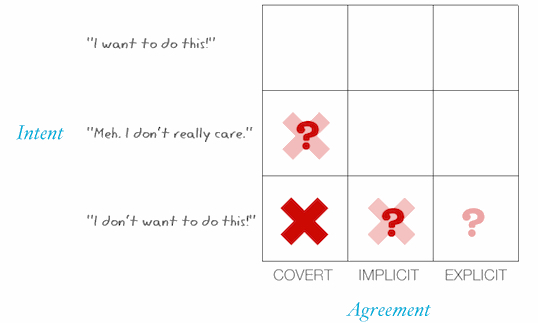
\includegraphics[width=\linewidth]{Resources/model.jpg}
  \caption{User Intent versus Agreement.}
  \label{fig:model}
\end{figure}

\subsection{Interfaces as Environments}

There is a tendency to describe UI design with the same terminology that one would use to design a service or a product. While the fundamentals are applicable in almost every area of design, it might be helpful to take a step back and consider the ways UI might be different. The word ``product'' implies a singular commodity, and is normally marketed or sold as a tool used to accomplish something. Service is defined as ``a facility supplying some public demand \cite{merriam-webster}.'' While both can be legitimately used for digital products, the terms are often lacking for the ways we describe user interfaces.

Architect turned designer Jorge Arango wrote a book entitled Living in Information to describe this problem. In it, he explores ways in which user interfaces should be considered information environments rather than products or services. Software like Facebook, Slack, or even macOS is more than a simple tool or product: it is a digital place where people interact with each other and spend (increasingly more) time. Arango says in chapter 6 that ``when your ''product`` is used for hours on end by billions of people every month, the thing you risk breaking is society itself. It’s time we recognize that these digital things we’re making are the places where many of our most important social interactions are happening, and start designing them accordingly. These things need architecture \cite{arango_2018}.''

Interface design that incorporates information architecture opens up many perspectives that are not typically considered in most product design, such as adaptability, accommodation, contextual coherence, and resilience to changing conditions. It places a greater emphasis on the fact that people create mental models from environmental clues in order to navigate their surroundings. Additionally, this view of design recognizes that the way an environment is architected facilitates the community around it, and how people utilize the space they are in.

Changing the designer's thinking from building a product to shaping a digital environment might lend greater weight to the influence they can have. Software is more than a singular tool; it is where the average adult spends nearly six hours of their lives every single day \cite{marvin_2018}.

\subsection{Christian Integration}

Up to this point, the moral implications of design have been applicable toward most any ethical framework. We will now explore how these findings have greater significance from the perspective of a Christian worldview.

\subsubsection{Design as Loving Neighbor}

The Christian faith observes that the first and greatest of all commandments is to ``love the Lord your God with all your heart and with all your soul and with all your mind,'' and the second to ``love your neighbor as yourself.'' On these two commandments, Jesus told the Pharisees, ``depend all the Law and the Prophets (Matt. 22:34-40 ESV).''

Christians can love their neighbors by integrating their faith into ethical interface design. The basic principles of UCD aligns well with this aspect of the law, as it places consideration of the end user's needs above the convenience of the developer. UCD is based upon an explicit understanding of the user and their tasks and environments, and requires an empathetic attitude toward their situation and emotions.

Loving neighbor properly requires looking at the broadest possible perspective of your user base. Just as ``there is no average user,'' there is no average neighbor. Each user will come with their own needs, backgrounds, and struggles. Each should be served by the interface in a way that is understandable and clear to them. Don Norman says that ``It is the duty of the machines and those who design them to understand people. It is not our duty to understand the arbitrary, meaningless dictates of machines \cite[p.~6]{norman_2013}.'' Truly understanding users requires respecting them as fellow bearers of God's image, not as cogs in the machine of the system.

True neighborly love does not bear false witness. Dark patterns that are designed to deceive, confuse, or manipulate the end user violate not only design principles, but the ninth commandment as well (Ex. 20:16).

\subsubsection{Design as Leadership}

As seen in the section that distinguished persuasion from manipulation, interface designers have a great responsibility to influence their end users toward some goal. As was quoted in that section, all design persuades behavior to some extent, and due to this we can see some commonalities between design and leadership. In essence, both leaders and designers have the duty to use all the power granted to them to guide their subjects to behave in a way that maximizes benefit for all involved (with the priority being the user or subject themselves).

Stated more specifically, the designer takes on the role of servant leader. While many forms of servant leadership exist outside of Christianity, the Biblical model is found by looking at the character and teachings of Jesus Christ recorded in Scripture. In Luke 22, Jesus compares the Gentile (unbelieving) kings with leaders that follow him: ``The kings of the Gentiles exercise lordship over them, and those in authority over them are called benefactors. But not so with you. Rather, let the greatest among you become as the youngest, and the leader as one who serves (Luke 22:25-26).'' This shows us that servant leaders are not benefactors from those they lead.

Further marks of a servant leader are demonstrated in the apostle Paul. His dedication to his duty was one that led him to forgo his own right rather than obscuring the gospel. He said to the Corinthian church that he made himself ``a servant to all,'' that he ``might win more of them (1 Cor. 9:19).'' He abstained from things that are not necessarily sinful (such as certain foods, drinks, marriage, or even financial support) if they could have potentially been stumbling blocks for those he was ministering to. Of course, service has different applications in the field of design than ministry, but the the central principles of good leadership remain intact. It is the responsibility of those who have influence over others to not only do no harm, but to positively promote good and influence upright behavior.

\subsubsection{Interfaces as Mediators}

Several times in this paper the concept of ``mediation'' has been mentioned. Mediation refers to the act of reconciling two or more parties, a removal of misunderstanding, or a conveyance of true understanding by means of an intermediary (or middleman). Interfaces function as mediators between end users and software systems, just as software itself functions as a mediator between humans and real life.

There is a corresponding theological idea when considering Jesus Christ as the mediator between God and mankind. Paul in his first letter to Timothy directly says this: ``For there is one God, and there is one mediator between God and men, the man Christ Jesus, who gave himself as a ransom for all, which is the testimony given at the proper time (1 Tim. 2:5-6).'' While there are obvious quantitative differences between user interfaces and the holy incarnate son of God, it is possible to learn some correlating qualities by seeing how Christ executes his office of mediator.

A good mediator effectively represents the interests of both parties. In his divine nature, Christ brings divine justice and mercy on his Father's behalf. In his human nature, Christ brings perfect obedience in fulfillment of the covenant of works made with Adam. Jesus, by means of his two distinguishable but inseparable natures, ``is able to save to the uttermost those who draw near to God through him, since he always lives to make intercession for them (Heb. 7:25).'' In a similar vein, user interfaces should always strive to effectively represent the interests of its users in a clear and consistent manner while simultaneously representing how the developer believes the software should be properly used.

UI designers should then see their role as creating and maintaining this mediation between users and software. Designers who live under Christian convictions have the ability to look to Jesus as the perfect example of one who represents the interests of both parties.

\section{Conclusion}

All software that is used by humans in any way requires an interface. All user interfaces involve design, and as we have shown, those design decisions affect every end user in some way. Design is persuasive by nature and can take any form, whether visual, audible, or sensory. Through several sources we have shown the fundamental principles that are seen across all fields of design, as well as several characteristics that are found in effective user interfaces. Due to the fact that interfaces are often meant to reduce the need for conscious effort (the ``don't make me think'' principle), it is imperative that designers make decisions with intentionality and consider all ethical ramifications.

The onslaught of dark patterns found in interfaces is not a recent phenomenon, but has become more relevant and dangerous as technology encroaches more into our everyday lives. It is up to users and developers working in tandem to design ethical, usable, and beautiful interfaces. Users should strive to be mindful of how they use software, should reward developers that respect their time and attention, and should reprove developers who do not. Developers must recognize recognize the potential vulnerability of their users and the influence that design has on their behavior, and fight against the temptation to implement user-hostile and metrics-driven dark patterns.

From the perspective of Christian ethics, one can view interface design as a unique opportunity to love neighbor, be a servant leader, and act as a mediator, all of which are ways that we can be further conformed to the image of Christ.

\newpage

\begingroup
\raggedright
\Urlmuskip=0mu plus 1mu\relax

\bibliography{SIP} 
\bibliographystyle{IEEEtran}

\endgroup

\end{document}  

















